\documentclass[11pt,UTF8]{article}
\usepackage[no-math,cm-default]{fontspec}
\usepackage{amsmath}
\usepackage{amsthm}
\usepackage{amssymb}
\usepackage{xeCJK}
\usepackage{verbatim}
\usepackage{indentfirst}
\usepackage{syntonly}
\usepackage{fancyhdr}
\usepackage[unicode=true, colorlinks, linkcolor=black, anchorcolor=black, citecolor=black, urlcolor=black]{hyperref}
\usepackage{graphicx}
\usepackage[top = 1.2in, bottom = 1.2in, left = 1.3in, right = 1.3in]{geometry}
\usepackage{xcolor}
\usepackage{paralist}
\usepackage{ulem}
\usepackage{titlesec}
\usepackage{zhspacing}
\usepackage{booktabs}
\usepackage{multirow}
\usepackage{supertabular}
\usepackage{float}
\usepackage{soul}
\usepackage{longtable}
\usepackage{listings}
\usepackage{xcolor}
\usepackage{multicol}
\lstset{
	numbers=left, 
	numberstyle= \tiny, 
	keywordstyle= \color{ blue!70},
	commentstyle= \color{red!50!green!50!blue!50}, 
	frame=shadowbox, % 阴影效果
	rulesepcolor= \color{ red!20!green!20!blue!20} ,
	escapeinside=``, % 英文分号中可写入中文
	xleftmargin=2em,xrightmargin=2em, aboveskip=1em,
	framexleftmargin=2em
} 
\setmainfont{Calibri}
\defaultfontfeatures{Mapping=tex-text}
%\setromanfont{Times New Roman}
%\newfontfamily\zhfont[BoldFont=Adobe Heiti Std]{Adobe Song Std}
\setmonofont[Scale=1]{Courier New}
\XeTeXlinebreaklocale "zh"
\XeTeXlinebreakskip = 0pt plus 1pt

\definecolor{hlcolor}{rgb}{0.9, 0.9, 0.9}
\sethlcolor{hlcolor}
\newcommand{\code}[1]{\texttt{\hl{#1}}}

\newcommand{\hlink}[1]{
	\footnote{\href{#1}{\textsl{\underline{#1}}}}
}
\renewenvironment{proof}{\noindent{\textbf{证明:}}}{\hfill $\square$ \vskip 4mm}
\newtheorem{conclusion*}{结论}
\newcommand{\conclusion}[1]{
	\begin{conclusion*}\textup{#1}\end{conclusion*}
}
\let\enumerate\compactenum
\let\endenumerate\endcompactenum
\let\itemize\compactitem
\let\enditemize\endcompactitem
\setlength{\pltopsep}{5pt}
\setlength{\parindent}{2em}
\setlength{\footskip}{30pt}
\setlength{\baselineskip}{1.3\baselineskip}
\renewcommand\arraystretch{1.2}

\lstset{language=C++,
	backgroundcolor=\color{hlcolor},
	extendedchars=false,
	basicstyle=\ttfamily,
	keywordstyle=\bfseries,
	commentstyle=\itshape\color{gray},
	escapeinside=`'}

\title{\fontsize{25pt}{\baselineskip}\textbf{数算实习大作业\\[2ex]验证码识别\ 实验报告}}
\author{陈志翰,胡家琛,李尚敏,周尚彦}
%\date{}

\pagestyle{fancy}
\renewcommand{\sectionmark}[1]{\markright{\thesection.\ #1}}
\renewcommand{\subsectionmark}[1]{}
%\fancyhead[C]{\small 湖南师大附中}
\fancyhead[L]{\small\slshape 验证码识别}
\fancyhead[R]{\small\slshape\nouppercase{\rightmark}}
\fancypagestyle{plain}{\fancyhead{}\fancyfoot{}\renewcommand{\headrulewidth}{0pt}}

\newcommand{\graph}[2]
{
\begin{figure}[H]
	\centering
	\includegraphics[width=\textwidth]{#1}
	\caption{#2}
\end{figure}
}

\begin{document}

\thispagestyle{plain}

\maketitle

%\setcounter{tocdepth}{1}
%\renewcommand{\contentsname}{\LARGE 目录}
\tableofcontents

\pagenumbering{arabic}
\setcounter{section}{0}

\section{算法简介}
\subsection{主要流程}
	\begin{enumerate}
	\item 实现一个简单的验证码生成算法,并利用该算法生成训练数据集与测试数据集
	\item 将训练集中验证码进行降噪处理
	\item 将降噪后的验证码切割为只含有单个字符的统一大小的图片
	\item 使用神经网络对训练数据集进行训练
	\item 对测试数据集使用相同的算法进行降噪与分割
	\item 使用处理后的测试数据集验证模型的准确度
	\end{enumerate}

\newpage
\subsection{验证码生成}
\paragraph{算法目的}
	每次以大小写字母与数字作为字符集,生成包含4个字符的验证码图片。

	利用该算法生成的验证码具有以下特点:
	\begin{enumerate}
	\item 字符相较标准字体有一定角度的偏移与形变
	\item 加入了噪点与干扰线以干扰识别
	\item 对图片进行了反走样处理与平滑处理,加大了识别难度
	\end{enumerate}
\paragraph{算法过程}
	\begin{enumerate}
	\item 随机生成一个四字字符串
	\item 调用PIL.ImageDraw的text方法 将DroidSansMono字体中的字以随机大小打在图片上
	\item 生成噪点
		\begin{enumerate}
		\item 随机$n$(设置为30)个坐标
		\item 对于每个坐标将其与其左上角坐标以画一条宽度为$width$(设置为3)的连线
		\end{enumerate}
	\item 随机两个坐标并将其连线作为干扰线
	\item 扭曲处理:
		\begin{enumerate}
		\item 随机一个偏移角度,计算出新图片的四个顶点的位置
		\item 对四个顶点加入随机的偏移量
		\item 调用PIL.Image的QUAD方法生成扭曲后的图片
		\end{enumerate}
	\item 调用PIL.ImageFilter将图片平滑处理
	\end{enumerate}
\newpage
\paragraph{算法示例}
	利用该算法生成的验证码示例如下:
	\begin{figure}[H]
		\centering
		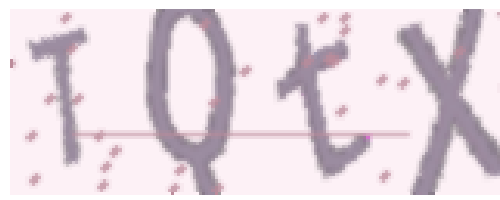
\includegraphics[width=\textwidth]{TQtx.png}
		\caption{验证码示例}\label{results}
	\end{figure}
	\begin{figure}[H]
		\centering
		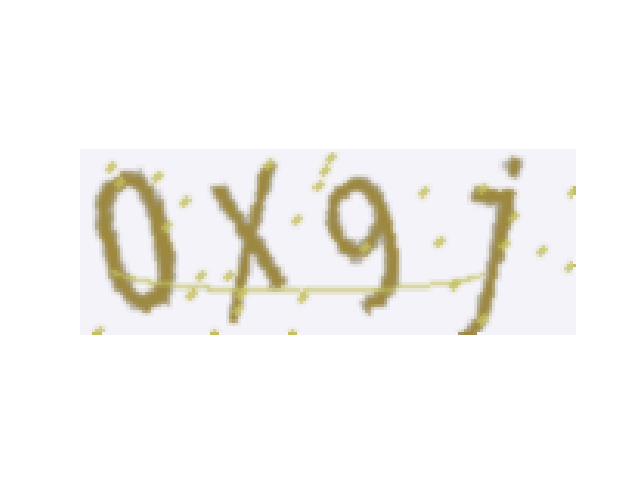
\includegraphics[width=\textwidth]{0X9j.png}
		\caption{验证码示例}\label{results}
	\end{figure}
\newpage
\subsection{降噪与切割处理}
\paragraph{算法目的}
	每次调用是读入给定验证码图片的rgba矩阵,并将其二值化
	(被视为背景与噪音的像素点为0,被视为字符的像素点为1)。
	
	之后将其切割成仅包含单个字符的统一大小的01矩阵作为返回值。

	该算法的难点在于
	\begin{enumerate}
	\item 各个字符大小不相同,分割的宽度也不相同
	\item 反走样处理使得字符上rgb值差异较大
	\item 平滑处理缩小了背景、噪音、字符的rgb值的差异
	\end{enumerate}
\paragraph{算法流程}
	\begin{enumerate}
	\item 读入验证码图片的rgb矩阵
	\item 将rgb分块处理,即将rgb值全除以8
	\item 首先在矩阵中找出出现最多的颜色块,作为标准背景颜色块
	\item 噪音和平滑处理会使得背景颜色驳杂,故将出现的
		行数次数之和大于$width*3/5$的颜色块则设为背景颜色块
	\item 在所有不为背景颜色中求出出现次数最多的颜色块,作为标准字符颜色块
	\item 寻找与标准颜色块相近的像素点,也视作字符颜色
	\item 寻找切割字符像素点较少的垂直线段作为切割线(加入距离筛选),切割图片
	\end{enumerate}
\newpage
\paragraph{算法示例}
	(降噪效果仅体现在二值化矩阵上,在原图中并未体现)

	\begin{figure}[H]
		\centering
		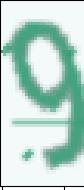
\includegraphics[width=0.2in]{9.png}
		\caption{字符切割示例}\label{results}
	\end{figure}
	\begin{figure}[H]
		\centering
		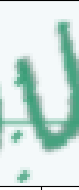
\includegraphics[width=0.2in]{U.png}
		\caption{字符切割示例}\label{results}
	\end{figure}
	\begin{figure}[H]
		\centering
		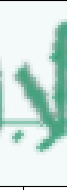
\includegraphics[width=0.2in]{y.png}
		\caption{字符切割示例}\label{results}
	\end{figure}
	\begin{figure}[H]
		\centering
		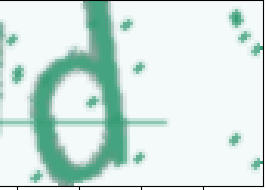
\includegraphics[width=0.2in]{d.png}
		\caption{字符切割示例}\label{results}
	\end{figure}
\newpage
\subsection{神经网络}
\paragraph{主要思路} 采用卷积神经网络进行图像识别。

\paragraph{数据预处理} 如上文所述,在降噪步骤中先将图像做0/1 normalization(二值化),将字符设置为1,噪音和背景设置为0
	(这样的normalization是很有必要且很有效果的),得到$30 \times 30$的01矩阵。

\paragraph{网络结构} 网络结构为:
	\begin{itemize}
	\item two convolutional layers 
	\item two fully connected layers.
	\end{itemize}

	两个conv layer分别拥有32和64个kernel,
	其中receptive field分别为$5 \times 5$和$3 \times 3$,
	使用ReLU作为activation。
	两个conv layer之后跟着一个max pooling layer,
	其中stride是$2$,filter size是$3 \times 3$,
	注意到这里我们使用了filter之间overlap的策略。

	为了防止overfitting,同时因为模型容量不需要太大,
	fully connected layer的数目比较少。
	两个fully connected layer均使用ReLU作为activation。
	Loss函数使用prediction和label之间
	(两个distribution之间)的cross entropy,即:
	$$H(L,p) = -\sum_x L(x) \log p(x)$$
	其中$p$由输出层(36个neuron,分别表示0-9和a-z)做softmax得到。
	softmax函数为:
	$$p(x) = \frac{e^x}{\sum_x e^x}$$
\paragraph{训练方式} 使用SGD算法进行训练,
	每个batch由100张验证码图片进行分割、降噪之后的数组组成
	在训练过程中忽略分割失败的数据。

\paragraph{改进}
	\begin{enumerate}
	\item 经过实验后发现该模型仍然有一点overfitting,
	所以在两个fully connected layer之间加入了一个dropout随机丢弃一些neurons,
	dropout rate设为$0.5$。
	\item 在改进1的基础上,发现generalization err仍然有一些大,
	于是增强了数据以增强网络的泛化性能。
	\end{enumerate}
\newpage
\section{算法与模型性能分析}
\subsection{代码与运行环境}
	\begin{itemize}
	\item 硬件配置
		\begin{itemize}
		\item CPU: AMD Ryzen R5 1600X
		\item GPU: Nvidia GeForce GTX 1050TI
		\item Memory: DDR4 16G 2400MHZ
		\end{itemize}
	\item 操作系统:Windows 10(X64)
	\item Python版本:Anaconda提供的Python3.5.3
	\item Tensorflow相关
		\begin{itemize}
		\item Tensorflow 1.3
		\item CUDA Toolkit 8.0
		\item cuDNN v6.1
		\end{itemize}
	\end{itemize}
\subsection{验证码生成与切割算法}
	\begin{itemize}
	\item 验证码生成与切割一张图片的时间大约为0.3秒
	\item 在没有噪点的情况下,切割算法的成功率可以达到$98\%$以上
	\item 在加入噪点的情况下,切割算法的成功率约为$80\%$
	\end{itemize}
%\newpage
\subsection{神经网络模型}
\paragraph{无噪点数据集}
	使用上文所述算法去掉生成噪点和干扰线的步骤,生成无噪点数据集。
	
	以30个batch的数据作为训练数据,在40000steps(约十分钟)之后,对于训练数据集的识别准确率达到$99.92\%$。

	使用另外30个batch的数据作为测试数据,对测试数据集的识别准确率约为$92\%$。
\paragraph{一般数据集}
	使用上文所述算法生成一般数据集。

	将150个batch的数据分为三部分,并进行交叉训练。在280000steps(约三小时)之后,对于三组训练数据的识别准确率均在$91\%$左右。

	使用另外60个batch的数据作为测试数据,对测试数据集的识别准确率约为$80\%$。

\end{document}